%%%%%%%%%%%%%%%%%%%%%%%%%%%%%%%%%%%%%%%%%
% Beamer Presentation
% LaTeX Template
% Version 2.0 (March 8, 2022)
%
% This template originates from:
% https://www.LaTeXTemplates.com
%
% Author:
% Vel (vel@latextemplates.com)
%
% License:
% CC BY-NC-SA 4.0 (https://creativecommons.org/licenses/by-nc-sa/4.0/)
%
%%%%%%%%%%%%%%%%%%%%%%%%%%%%%%%%%%%%%%%%%

%----------------------------------------------------------------------------------------
%	PACKAGES AND OTHER DOCUMENT CONFIGURATIONS
%----------------------------------------------------------------------------------------
\documentclass[
  24pt, % Set the default font size, options include: 8pt, 9pt, 10pt, 11pt, 12pt, 14pt, 17pt, 20pt
  %t, % Uncomment to vertically align all slide content to the top of the slide, rather than the default centered
  aspectratio=169, % Uncomment to set the aspect ratio to a 16:9 ratio which matches the aspect ratio of 1080p and 4K screens and projectors
]{beamer}

\graphicspath{{Images/}{./}} % Specifies where to look for included images (trailing slash required)

\usepackage{booktabs} % Allows the use of \toprule, \midrule and \bottomrule for better rules in tables

%----------------------------------------------------------------------------------------
%	SELECT LAYOUT THEME
%----------------------------------------------------------------------------------------

% Beamer comes with a number of default layout themes which change the colors and layouts of slides. Below is a list of all themes available, uncomment each in turn to see what they look like.

%\usetheme{default}
%\usetheme{AnnArbor}
%\usetheme{Antibes}
%\usetheme{Bergen}
%\usetheme{Berkeley}
%\usetheme{Berlin}
\usetheme{Boadilla} %me gusta
%\usetheme{CambridgeUS}
%\usetheme{Copenhagen}
%\usetheme{Darmstadt}
%\usetheme{Dresden}
%\usetheme{Frankfurt}
%\usetheme{Goettingen} %dos dos
%\usetheme{Hannover} %dos dos
%\usetheme{Ilmenau}
%\usetheme{JuanLesPins}
%\usetheme{Luebeck}
%\usetheme{Madrid}
%\usetheme{Malmoe}
%\usetheme{Marburg}
%\usetheme{Montpellier}
%\usetheme{PaloAlto}
%\usetheme{Pittsburgh}
%\usetheme{Rochester} %muy flat
%\usetheme{Singapore}
%\usetheme{Szeged}
%\usetheme{Warsaw}

%----------------------------------------------------------------------------------------
%	SELECT COLOR THEME
%----------------------------------------------------------------------------------------

% Beamer comes with a number of color themes that can be applied to any layout theme to change its colors. Uncomment each of these in turn to see how they change the colors of your selected layout theme.

%\usecolortheme{albatross}
%\usecolortheme{beaver}
%\usecolortheme{beetle}
%\usecolortheme{crane}
%\usecolortheme{dolphin}
%\usecolortheme{dove}
%\usecolortheme{fly}
%\usecolortheme{lily} %default
%\usecolortheme{monarca}
%\usecolortheme{seagull}
%\usecolortheme{seahorse}
%\usecolortheme{spruce}
%\usecolortheme{whale}
%\usecolortheme{wolverine}

%----------------------------------------------------------------------------------------
%	SELECT FONT THEME & FONTS
%----------------------------------------------------------------------------------------

% Beamer comes with several font themes to easily change the fonts used in various parts of the presentation. Review the comments beside each one to decide if you would like to use it. Note that additional options can be specified for several of these font themes, consult the beamer documentation for more information.

\usefonttheme{default} % Typeset using the default sans serif font
%\usefonttheme{serif} % Typeset using the default serif font (make sure a sans font isn't being set as the default font if you use this option!)
%\usefonttheme{structurebold} % Typeset important structure text (titles, headlines, footlines, sidebar, etc) in bold
%\usefonttheme{structureitalicserif} % Typeset important structure text (titles, headlines, footlines, sidebar, etc) in italic serif
%\usefonttheme{structuresmallcapsserif} % Typeset important structure text (titles, headlines, footlines, sidebar, etc) in small caps serif

%------------------------------------------------

%\usepackage{mathptmx} % Use the Times font for serif text
\usepackage{palatino} % Use the Palatino font for serif text

\usepackage[ruled,vlined]{algorithm2e}
%\usepackage{helvet} % Use the Helvetica font for sans serif text
\usepackage[default]{opensans} % Use the Open Sans font for sans serif text
\usepackage[spanish]{babel}
\usepackage{dirtree}
\usepackage{xcolor}
%\usepackage[default]{FiraSans} % Use the Fira Sans font for sans serif text
%\usepackage[default]{lato} % Use the Lato font for sans serif text

\usepackage[scaled]{helvet}
\usepackage[round]{natbib}
%\newcommand{\newblock}{}

\usepackage{rotating}

\newcommand\FourQuad[4]{%
  \begin{minipage}[b][.33\textheight][t] 
    {.48\textwidth}#1\end{minipage}\hfill%
    \begin{minipage}[b][.33\textheight][t] 
      {.48\textwidth}#2\end{minipage}\\[0.5em]
      \begin{minipage}[b][.33\textheight][t] 
        {.48\textwidth}#3\end{minipage}\hfill
        \begin{minipage}[b][.33\textheight][t] 
          {.48\textwidth}#4\end{minipage}%
}

\usepackage{tikz}
%\usetikzlibrary{arrows,shapes,positioning,shadows,trees,quotes}


%\tikzset{
%  basic/.style  = {draw, text width=2cm, drop shadow, font=\sffamily, rectangle},
%  root/.style   = {basic, rounded corners=2pt, thin, align=center,
%                   fill=green!30},
%  level 2/.style = {basic, rounded corners=6pt, thin,align=center, fill=green!60,
%                   text width=8em},
%  level 3/.style = {basic, thin, align=left, fill=pink!60, text width=6.5em}
%}

\usetikzlibrary{calc}

\tikzstyle{part} = [rectangle, rounded corners, minimum width=3cm, minimum height=1cm,     align=center, draw=black]
\tikzstyle{chapter} = [rectangle, rounded corners, minimum width=3cm, minimum height=1cm,     align=center, draw=black, text width=3.5cm]
\tikzstyle{arrow} = [thick, ->]

\usepackage{array} % needed for \arraybackslash
\usepackage{graphicx}
\usepackage{adjustbox} % for \adjincludegraphics

\usepackage{subcaption}
\usepackage{bibentry}
%\bibliographystyle{apalike}
\usepackage{chngcntr}
\usepackage{lipsum}% http://ctan.org/pkg/lipsum
\usepackage{hanging}% http://ctan.org/pkg/hanging

\usepackage{xcolor,colortbl}
\usepackage{multirow}

\usepackage{animate}
\usepackage{multicol}
\usepackage{tabularx,booktabs}
\usepackage{forloop}
\usepackage{ragged2e}

\usepackage{bbding} %palomitas checkmark
\usepackage{pifont}
\usepackage{lipsum,tabularx}
\newcounter{loopcntr}
%----------------------------------------------------------------------------------------
%	SELECT INNER THEME
%----------------------------------------------------------------------------------------

% Inner themes change the styling of internal slide elements, for example: bullet points, blocks, bibliography entries, title pages, theorems, etc. Uncomment each theme in turn to see what changes it makes to your presentation.

%\useinnertheme{default}
\useinnertheme{circles}
%\useinnertheme{rectangles}
%\useinnertheme{rounded}
%\useinnertheme{inmargin}

%----------------------------------------------------------------------------------------
%	SELECT OUTER THEME
%----------------------------------------------------------------------------------------

% Outer themes change the overall layout of slides, such as: header and footer lines, sidebars and slide titles. Uncomment each theme in turn to see what changes it makes to your presentation.

%\useoutertheme{default}
%\useoutertheme{infolines}
%\useoutertheme{miniframes}
%\useoutertheme{smoothbars}
%\useoutertheme{sidebar}
%\useoutertheme{split}
%\useoutertheme{shadow}
%\useoutertheme{tree}
%\useoutertheme{smoothtree}

%\setbeamertemplate{footline} % Uncomment this line to remove the footer line in all slides
\setbeamertemplate{footline}[page number] % Uncomment this line to replace the footer line in all slides with a simple slide count
%\setbeamertemplate{caption}[numbered]
\setbeamertemplate{navigation symbols}{} % Uncomment this line to remove the navigation symbols from the bottom of all slides

%----------------------------------------------------------------------------------------
%	PRESENTATION INFORMATION
%----------------------------------------------------------------------------------------

\title[PROTOCOLO DE INVESTIGACIÓN]{%\centering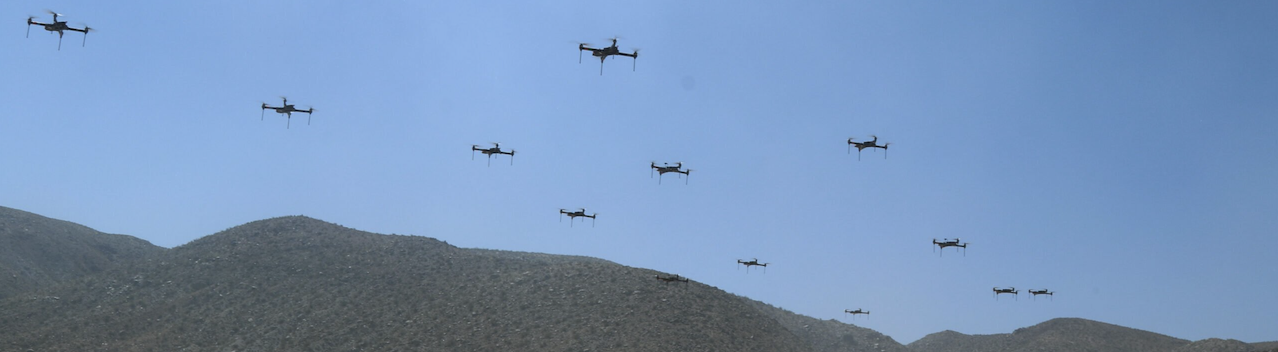
\includegraphics[width=10cm]{swarm_drones}\\
  Estrategias para la exploración coordinada multi-VANT} % The short title in the optional parameter appears at the bottom of every slide, the full title in the main parameter is only on the title page

%\subtitle{Optional Subtitle} % Presentation subtitle, remove this command if a subtitle isn't required

\author[Luis Ballado]{Luis Alberto Ballado Aradias} % Presenter name(s), the optional parameter can contain a shortened version to appear on the bottom of every slide, while the main parameter will appear on the title slide

\institute[CINVESTAV]{
  CINVESTAV UNIDAD TAMAULIPAS \\
  %\smallskip \textit{luis.ballado@cinvestav.mx}
} % Your institution, the optional parameter can be used for the institution shorthand and will appear on the bottom of every slide after author names, while the required parameter is used on the title slide and can include your email address or additional information on separate lines

\date[\today]{Cd. Victoria, Tamaulipas - \today} % Presentation date or conference/meeting name, the optional parameter can contain a shortened version to appear on the bottom of every slide, while the required parameter value is output to the title slide

%\titlegraphic{\hspace*{8.75cm}~%
%   
\includegraphics[width=0.8cm]{cinvestavlogo}
%}

%----------------------------------------------------------------------------------------

\counterwithin*{footnote}{page}
\newcommand\footcite[1]{\footnote{\bibentry{#1}}\label{\thepage:#1}}
\newcommand\secondcite[1]{\textsuperscript{\ref{\thepage:#1}}}

\newcommand{\rpt}[2][1]{%
  \forloop{loopcntr}{0}{\value{loopcntr}<#1}{#2}%
}
\newcommand{\on}[1][1]{
  \forloop{loopcntr}{0}{\value{loopcntr}<#1}{&\cellcolor{gray}}
}
\newcommand{\onok}[1][1]{
  \forloop{loopcntr}{0}{\value{loopcntr}<#1}{&\cellcolor{green}}
}
\newcommand{\off}[1][1]{
  \forloop{loopcntr}{0}{\value{loopcntr}<#1}{&\cellcolor{white}}
}

\addtolength{\textheight}{90pt}

\newcommand{\I}{\mathbb{I}}
\newcommand{\K}{\mathbb{K}}
\newcommand{\N}{\mathbb{N}}
\newcommand{\Q}{\mathbb{Q}}
\newcommand{\R}{\mathbb{R}}
\newcommand{\Z}{\mathbb{Z}}

\newcommand{\specialcell}[2][c]{%
  \begin{tabular}[#1]{@{}c@{}}#2\end{tabular}}


\begin{document}

%----------------------------------------------------------------------------------------
%	TITLE SLIDE
%----------------------------------------------------------------------------------------

\begin{frame}
  \titlepage % Output the title slide, automatically created using the text entered in the PRESENTATION INFORMATION block above
\end{frame}

%----------------------------------------------------------------------------------------
%	TABLE OF CONTENTS SLIDE
%----------------------------------------------------------------------------------------

% The table of contents outputs the sections and subsections that appear in your presentation, specified with the standard \section and \subsection commands. You may either display all sections and subsections on one slide with \tableofcontents, or display each section at a time on subsequent slides with \tableofcontents[pausesections]. The latter is useful if you want to step through each section and mention what you will discuss.
\AtBeginSection[]
{
  \begin{frame}
    \frametitle{Contenido} % Slide title, remove this command for no title
    \tableofcontents[currentsection] % Output the table of contents (all sections on one slide)
    %\tableofcontents[pausesections] % Output the table of contents (break sections up across separate slides)
  \end{frame}
}
%----------------------------------------------------------------------------------------
%	PRESENTATION BODY SLIDES
%----------------------------------------------------------------------------------------

\section{Antecedentes y motivación del proyecto}
\begin{frame}{Antecedentes}
  \bigskip % Vertical whitespace
  \centering
  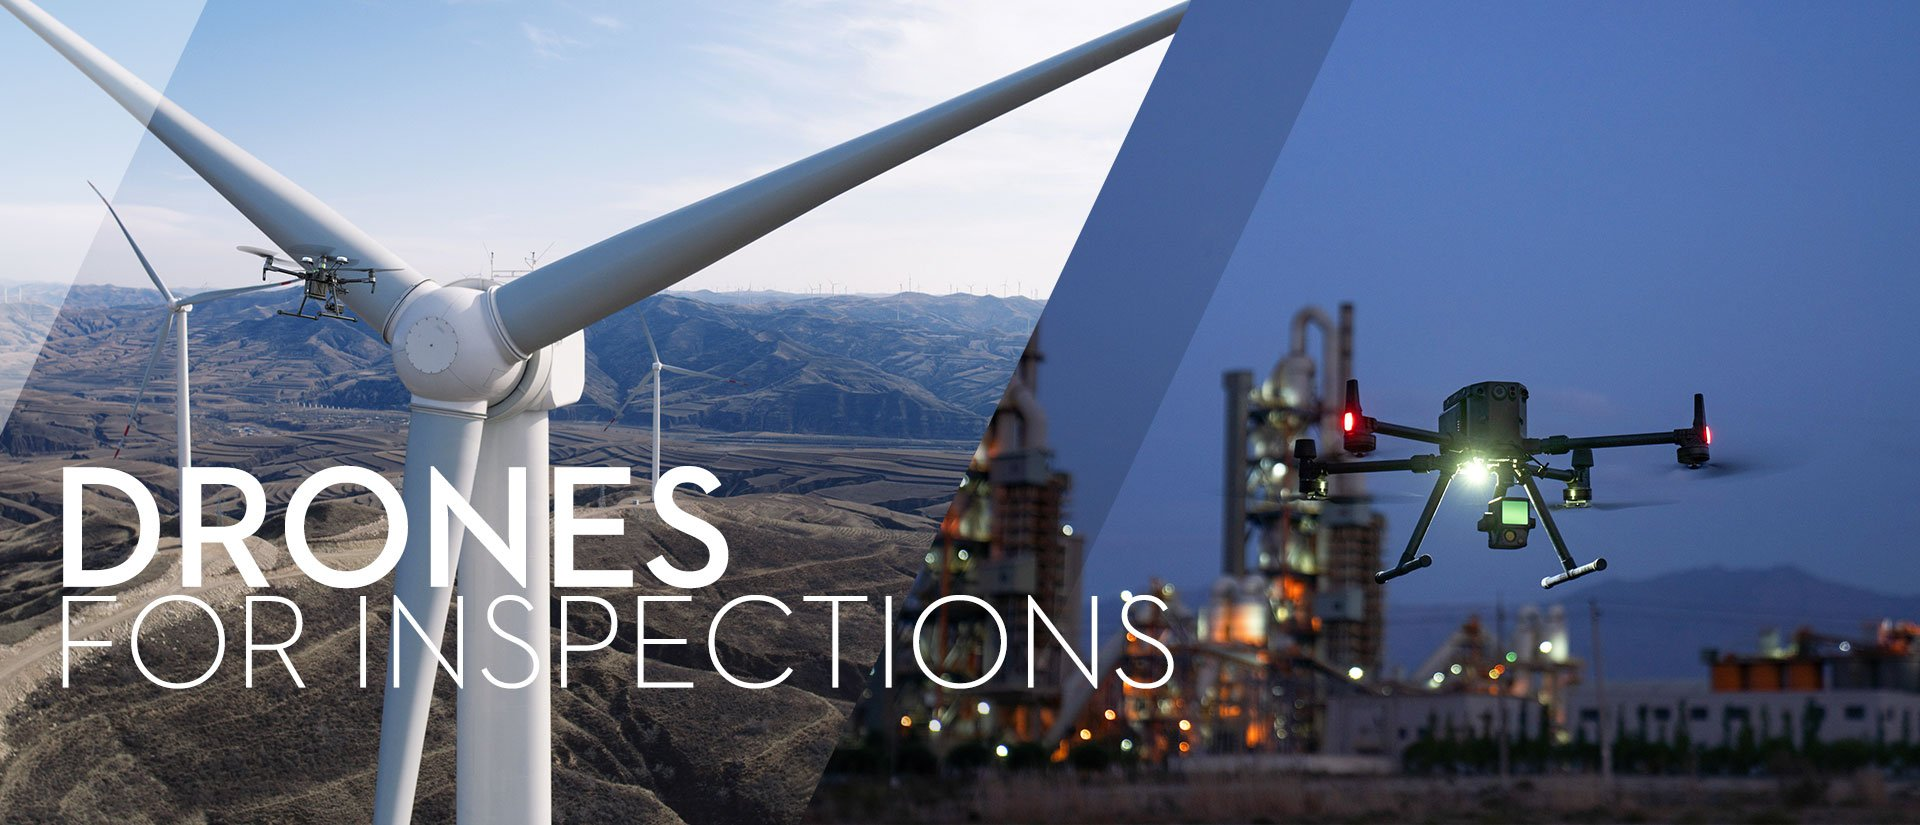
\includegraphics[width=0.45\textwidth,height=0.35\textheight]{DJI_B1}$^\dag$
  \hfil
  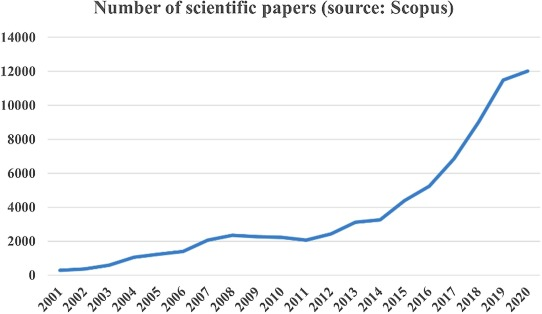
\includegraphics[width=0.45\textwidth,height=0.35\textheight]{survey_chart.jpg}\footnotemark
  \vspace{2pt}\\
  
  \begin{itemize}
  \item \textbf{Aplicaciones} en lugares inaccesibles o peligrosos.
  \item \textbf{Múltiples VANT} pueden reducir el tiempo de exploración y aumentar la confianza del sistema.
  \item \textbf{Limitaciones} en carga, procesamiento y batería influyen en el tiempo de vuelo.
  \end{itemize}

  \footnotetext{UAV in the advent of the twenties: Where we stand and what is next [\cite{Nex2022}]}
  %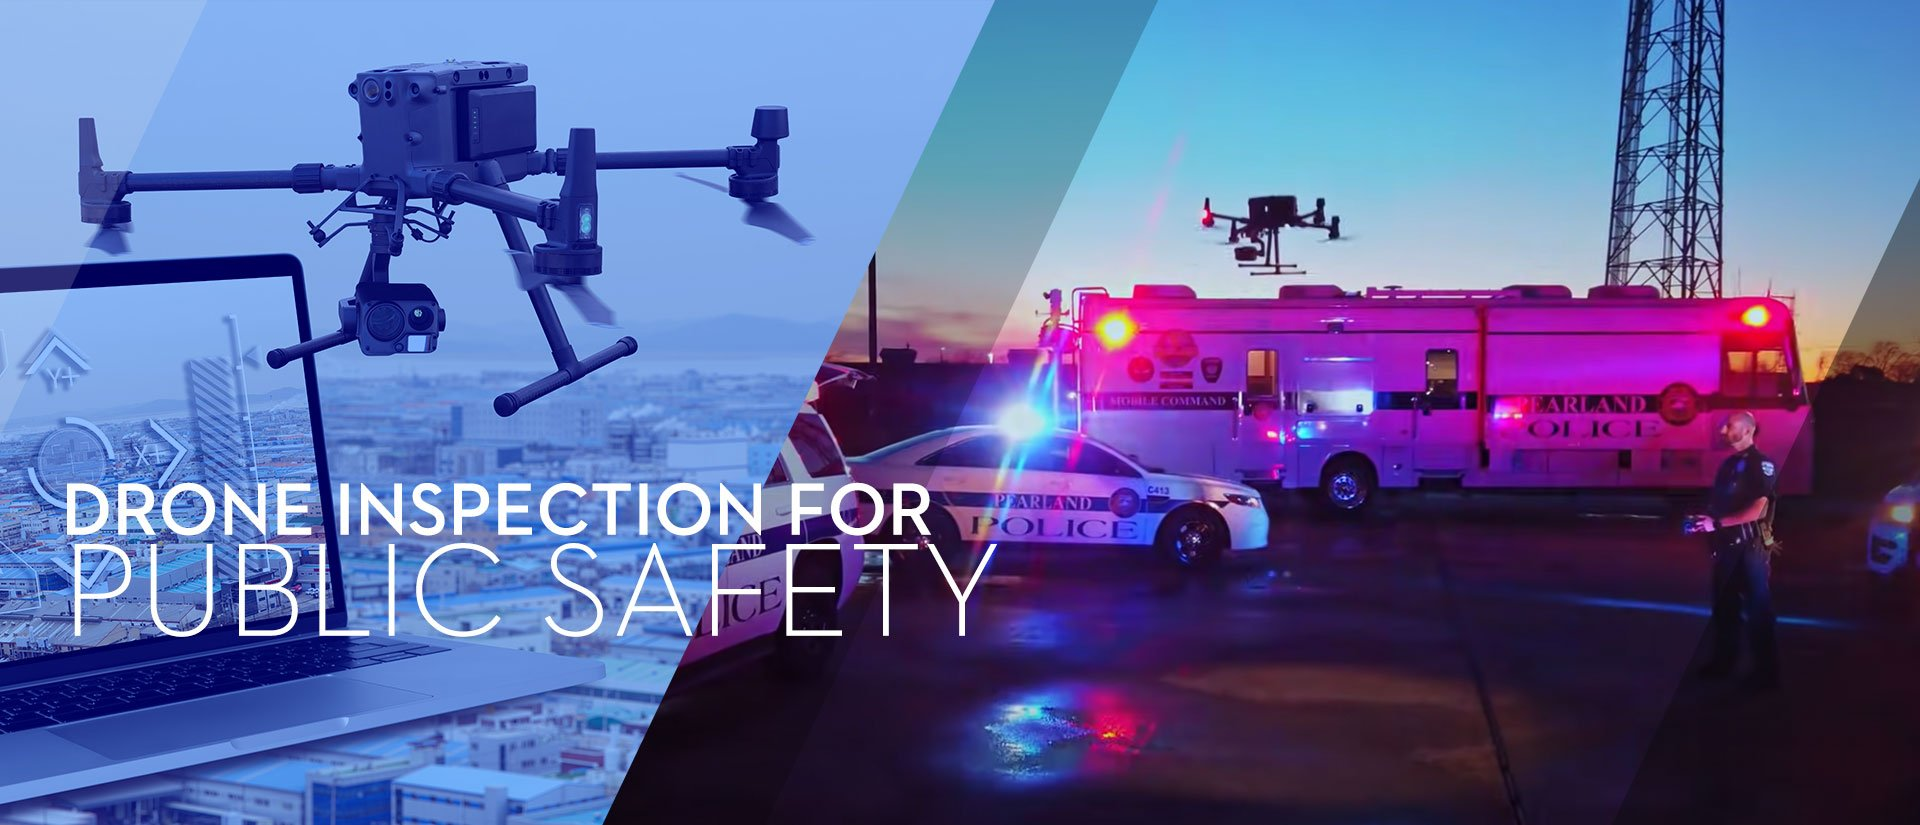
\includegraphics[width=0.45\textwidth,height=0.35\textheight]{DJI_B5}$^\dag$ 
  %\hfil
  %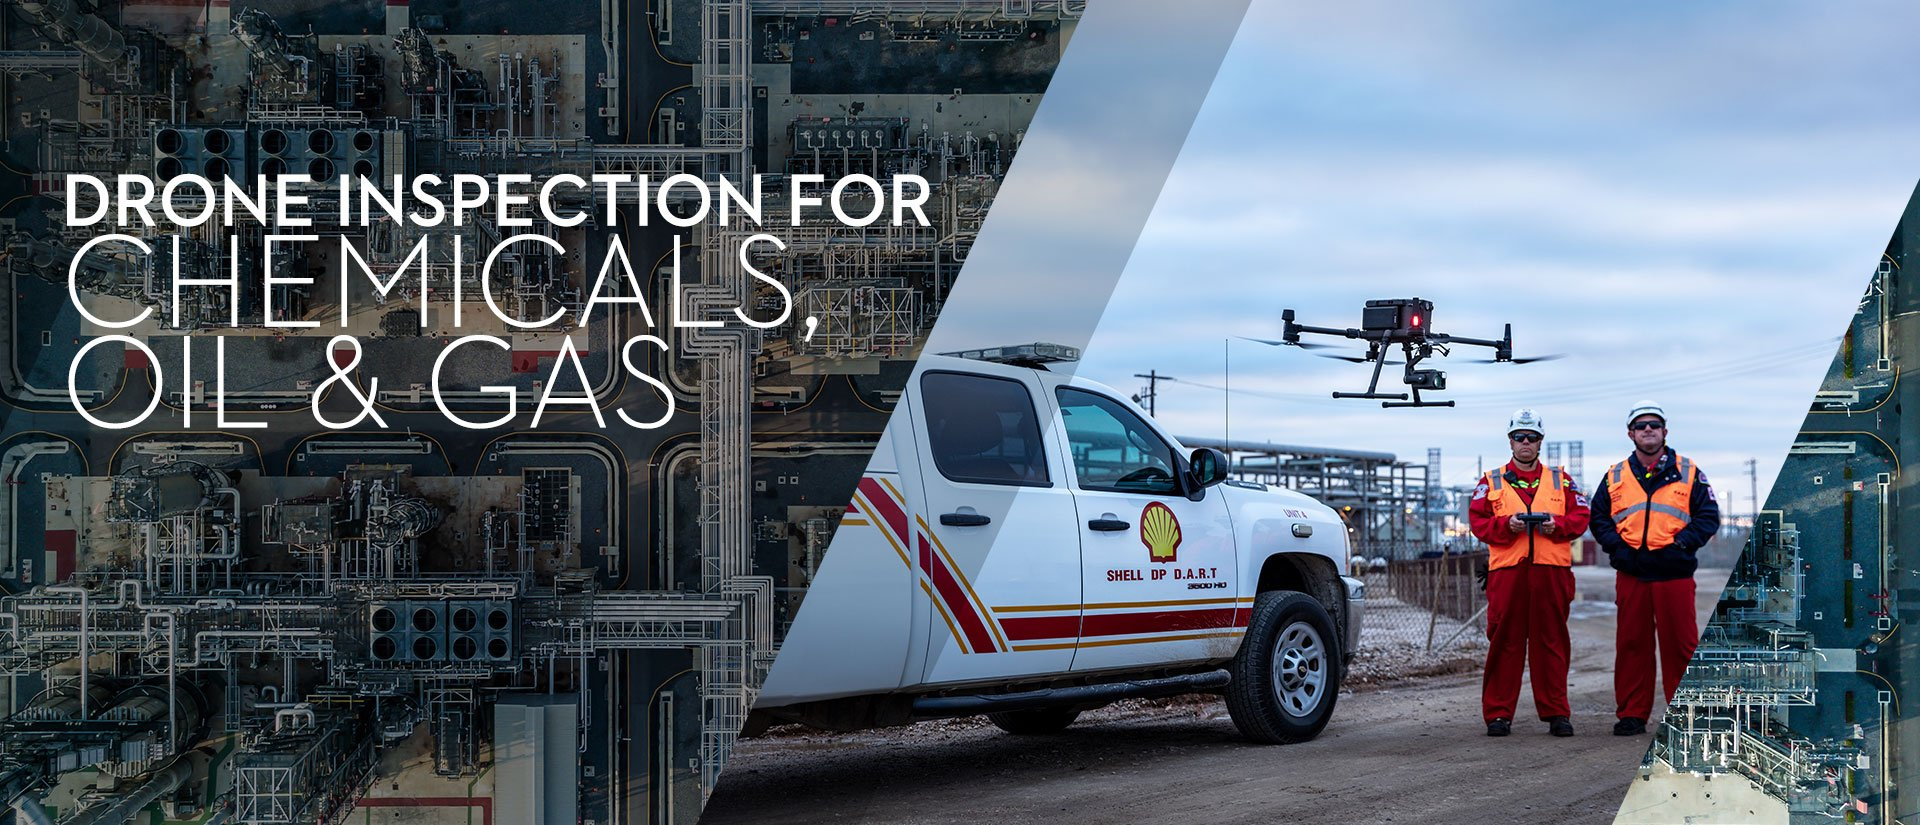
\includegraphics[width=0.45\textwidth,height=0.35\textheight]{DJI_B4}$^\dag$\\
  %\rule{0in}{1.2em}$^\dag$ \small Inspecciones con VANT basadas en los mejores casos de uso\\
  %\tiny \url{https://enterprise-insights.dji.com/blog/complete-guide-to-drone-inspections}
\end{frame}

\begin{frame}{Antecedentes}
  
  %\centering
  Principales preguntas que un robot autónomo debe responder \footnotemark
  \bigskip % Vertical whitespace
  \begin{itemize}
  \item ¿Dónde estoy? $\implies$ Localización 
  \item ¿A dónde voy? $\implies$ Cognición
  \item ¿Cómo llego hasta ahí? $\implies$ Planificación de trayectoria
  \end{itemize}
  \pause
  \bigskip % Vertical whitespace
  Para resolver estas preguntas, el robot debe:
  \bigskip % Vertical whitespace
  \begin{itemize}
  \item Tener un modelo del ambiente (dado, o autónomamente construido)
  \item Localizarse dentro del ambiente
  \item Planear y ejecutar los movimientos
  \end{itemize}

  \footnotetext{Visual map making for a mobile robot [\cite{1087348}]}
  
\end{frame}

\begin{frame}{Localización - ¿Dónde estoy?}

  Problema de Localización y Mapeo Simultáneos  \footnote{Simultaneous localization and mapping: part I [\cite{slam_doc}]}
  \bigskip % Vertical whitespace
  \begin{itemize}
    \item \textcolor{blue}{VER}: El Robot utiliza la lectura de sus sensores para encontrarse a el mismo.
      \bigskip % Vertical whitespace
    \item \textcolor{red}{ACTUAR}: El Robot, se mueve hacia adelante
      \begin{itemize}
      \item Movimiento estimado a partir de las lecturas de la odometría.
      \item Acumulación de incertidumbre.
      \end{itemize}
      \bigskip % Vertical whitespace
    \item \textcolor{blue}{VER}: Lectura de sus sensores nuevamente para localizarse a sí mismo
  \end{itemize}
      
  \bigskip % Vertical whitespace
  Belief update (Fusión de información) \footnote{Uncertain geometry in robotics [\cite{slam_dur}]} \footnote{Estimating Uncertain Spatial Relationships in Robotics [\cite{Smith1988}]}
  
\end{frame}

\begin{frame}{Cognición - ¿A dónde voy?}
  
  %\centering
  \begin{figure}[h]
    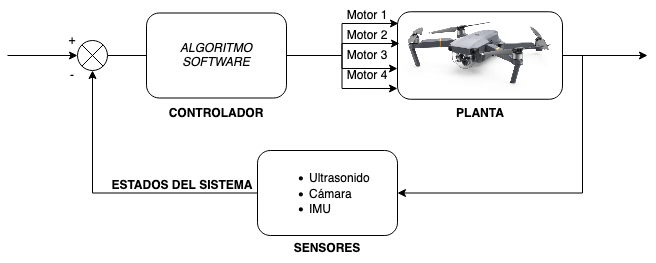
\includegraphics[width=0.65\textwidth]{control_drone.png}
    \caption{Diagrama control lazo cerrado VANT}
  \end{figure}
  \bigskip % Vertical whitespace
  \small Un sistema de control para un robot móvil autónomo opera en un entorno donde las condiciones están cambiando rápidamente. (considerando el problema de control instantáneo en una formulación clásica de teoría de control) \footnote{A robust layered control system for a mobile robot [\cite{brooks_robot}]}
  
\end{frame}

\begin{frame}{Arquitectura híbrida}
  \begin{minipage}{0.47\textwidth}
    
    \small El robot puede reaccionar de manera rápida a estímulos del entorno, al mismo tiempo que tiene la capacidad de planificar y tomar decisiones de alto nivel.
    
    \begin{itemize}
    \item Adaptable al lidiar con situaciones predecibles como imprevistas.
    \item Permite una respuesta rápida a estímulos del entorno.
    \item Optmiza el rendimiento del robot al gestionar las tareas simples y repetitivas, liberando recursos para tareas deliberativas más complejas.
    \item Es escalable.
    \end{itemize}
  \end{minipage}
  \hspace{0.2cm}
  \begin{minipage}{0.5\textwidth}
    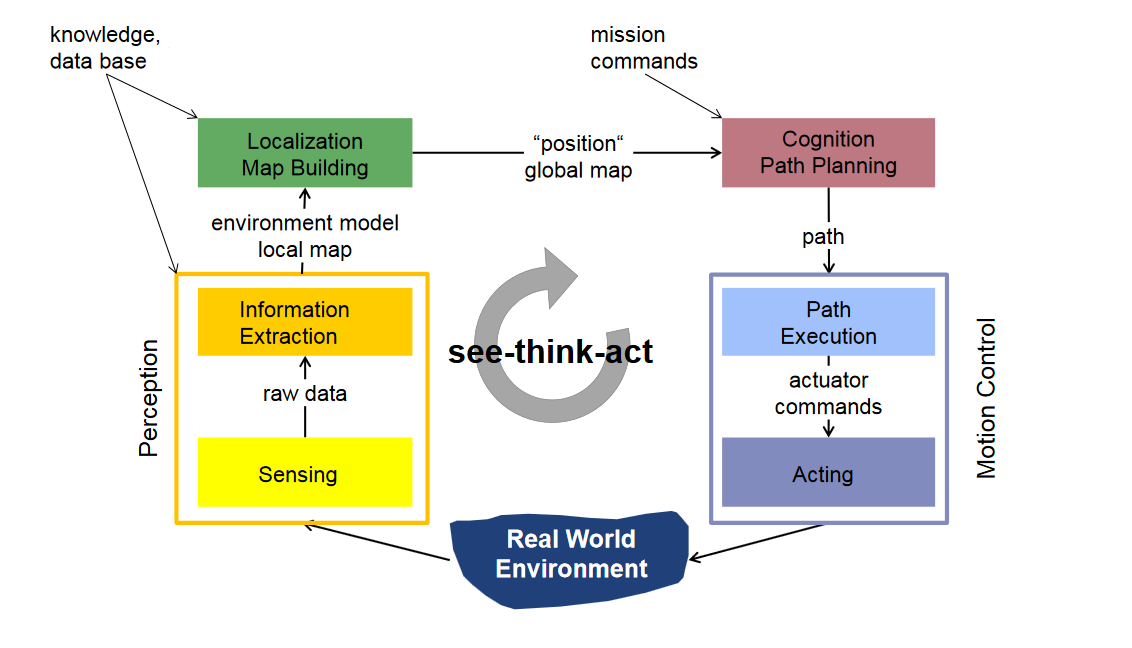
\includegraphics[width=\textwidth]{control-scheme}$^\dag$\\
    \rule{0in}{1.2em}$^\dag$\scriptsize Ciclo See-Think-Act \\
    \tiny ETH - Note Class Autonomous mobile robot 2015 
  \end{minipage}
\end{frame}

\begin{frame}{Planificación de trayectoria - ¿Cómo llego hasta ahí?}
  \begin{minipage}{0.57\textwidth}

    El uso de heuristicas para encontrar soluciones óptimas, proporciona resultados computacionales eficientes. \footnote{A Survey of Trajectory Planning Techniques for Autonomous Systems [\cite{Mir2022}]} 
    \bigskip % Vertical whitespace
    \begin{itemize}
    \item Planificador de trayectoria global
      \begin{itemize}
      \item Búsqueda por grafos
      \end{itemize}
      \bigskip % Vertical whitespace
    \item Planificador de trayectoria local
      \begin{itemize}
      \item Campos de potencial artifical
      \item Algoritmos Bug
      \end{itemize}
    \end{itemize}
    \bigskip % Vertical whitespace
  \end{minipage}
  \hspace{0.2cm}
  \begin{minipage}{0.4\textwidth}
    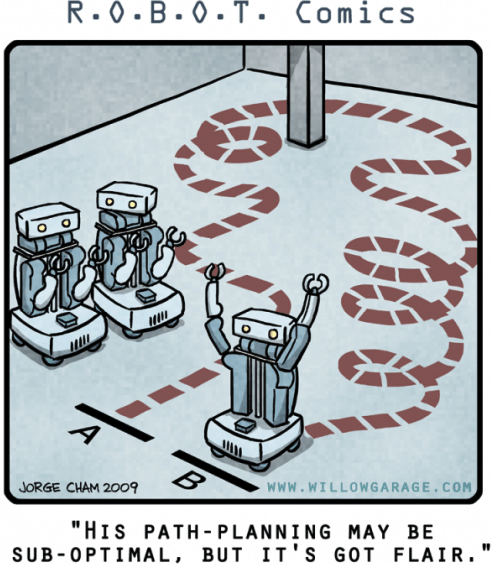
\includegraphics[width=0.6\textwidth]{img5}$^\dag$\\
  \end{minipage}
\end{frame}

%\begin{frame}{Vehículos aéreos no tripulados (VANT)}
%  \bigskip % Vertical whitespace
%  \centering
%  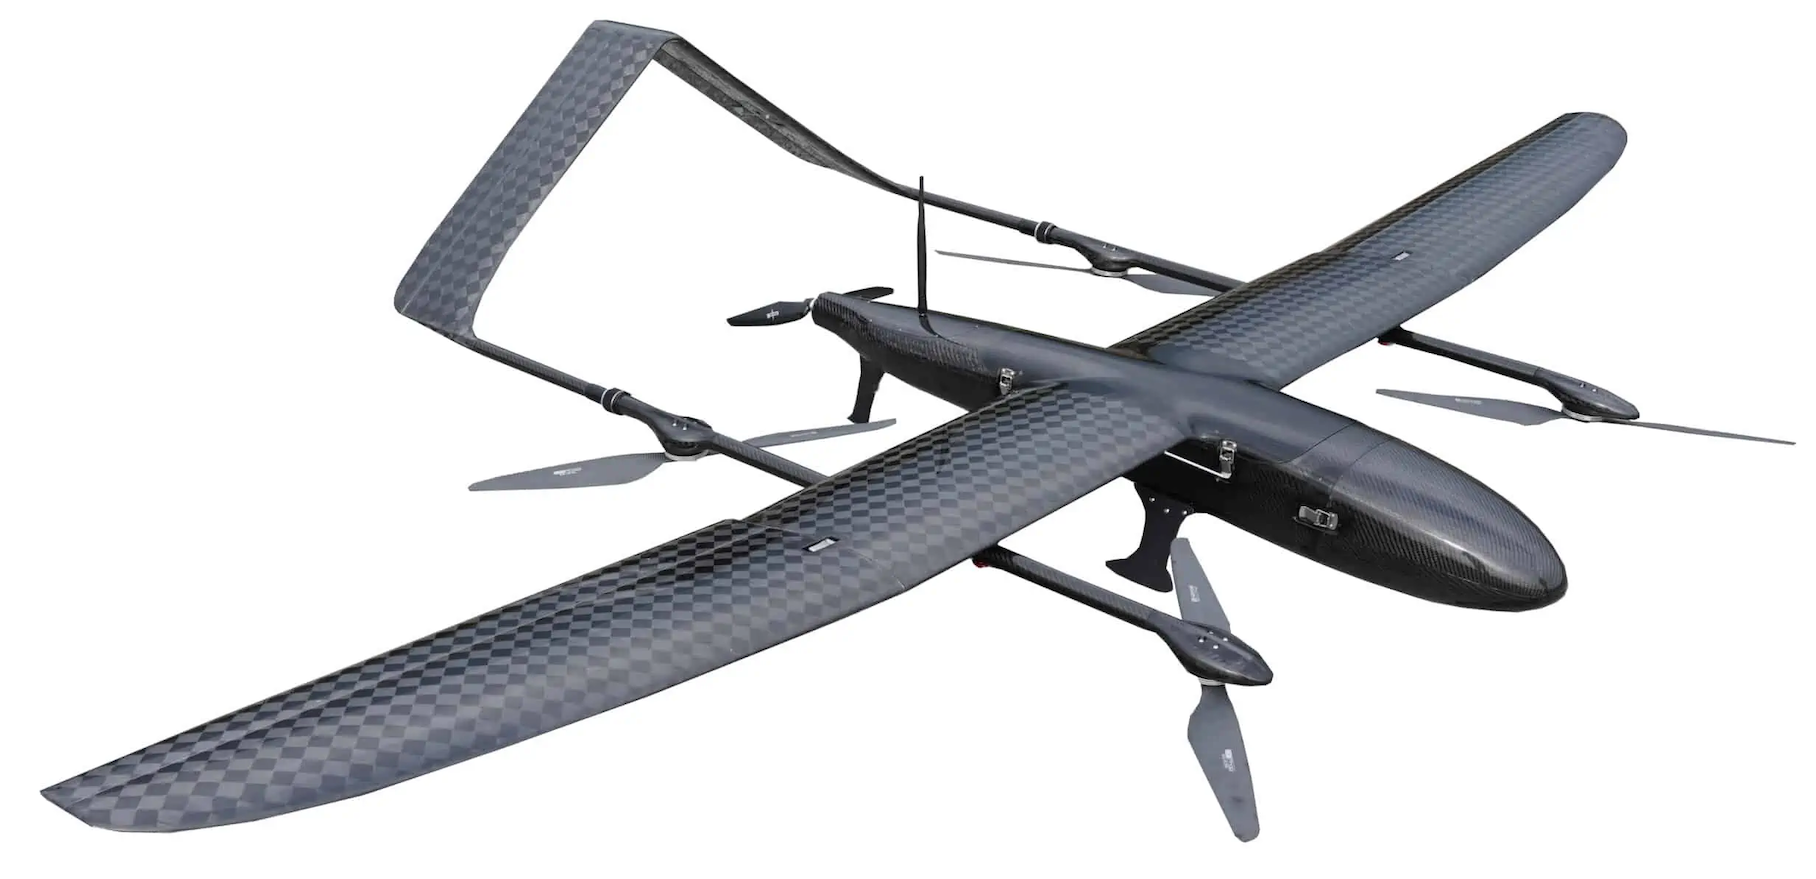
\includegraphics[width=0.45\textwidth,height=0.35\textheight]{img6}
%  \hfil
%  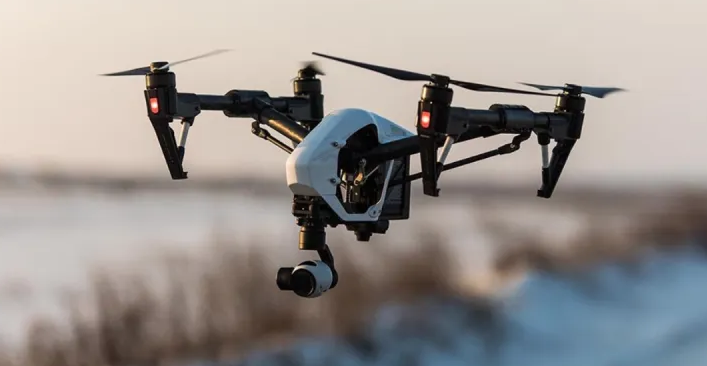
\includegraphics[width=0.45\textwidth,height=0.35\textheight]{img7}
%  \vspace{2pt}
%  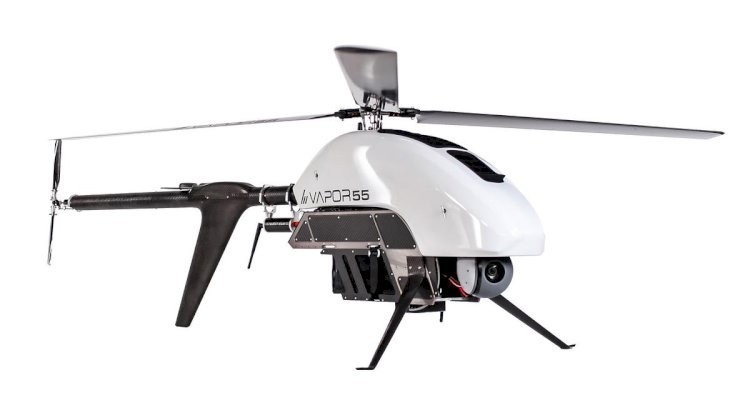
\includegraphics[width=0.45\textwidth,height=0.35\textheight]{img8.jpg}
%  \hfil
%  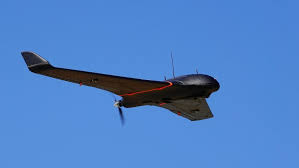
\includegraphics[width=0.45\textwidth,height=0.35\textheight]{img9.jpg}
%  \rule{0in}{1.2em} \small Clasificación VANTS \\
%  \tiny  Handbook of Unmanned Aerial Vehicles 2020
%\end{frame}

%\begin{frame}{Sistema autónomo VANT}
%  \begin{minipage}{0.47\textwidth}
    
%    \small Un sistema autónomo de un vehículo aéreo no tripulado consta de tres algoritmos.
    
%    \begin{itemize}
%    \item Generación de una representación del entorno.
%    \item Evasión de obstáculos.
%    \item Planificación de trayectorias.
%    \end{itemize}

%    \small La computadora embebida usado en un micro-VANT es de bajo rendimiento, pero su necesidad de autónomia sigue siendo la misma que un VANT de mayor tamaño.\\
%    Es necesario dotarlos de algoritmos de baja complejidad computacional.
    
%  \end{minipage}
%  \hspace{0.2cm}
%  \begin{minipage}{0.5\textwidth}
%    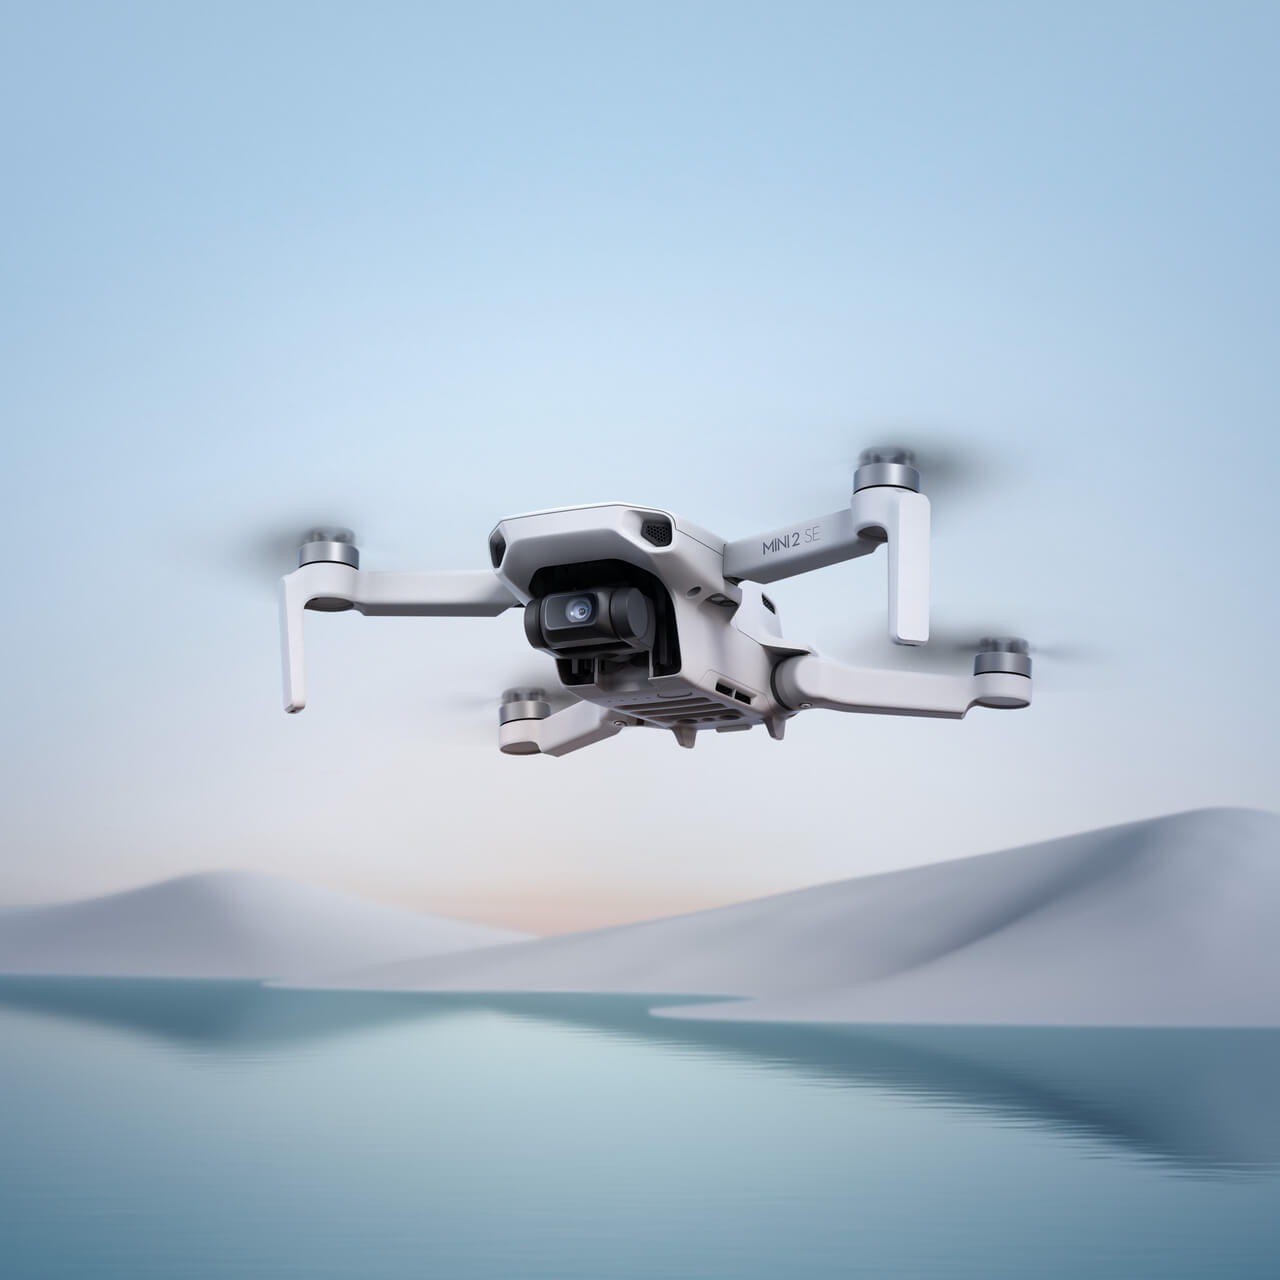
\includegraphics[width=\textwidth]{ultra.jpg}
%  \end{minipage}
%\end{frame}


%\begin{frame}{Generación de mapas}
%  \bigskip % Vertical whitespace
  %\centering
%  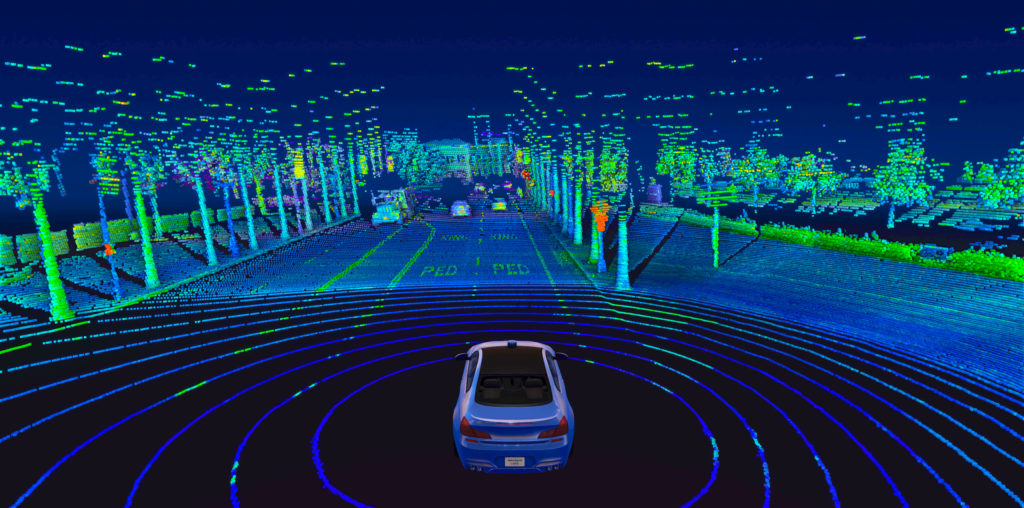
\includegraphics[width=0.45\textwidth,height=0.35\textheight]{map3d.jpg}$^\dag$
%  \hfil
%  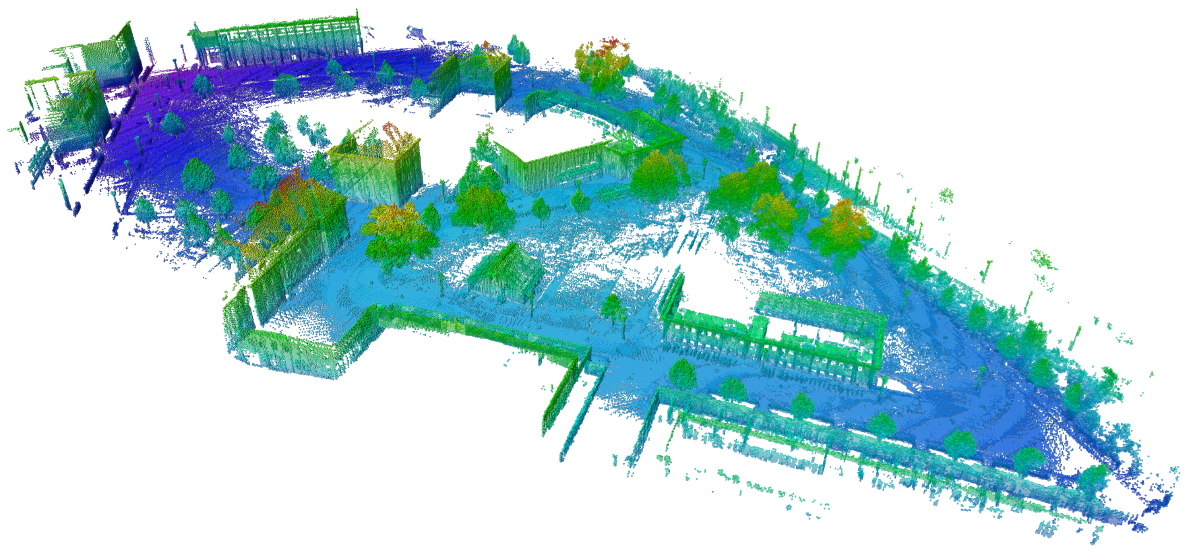
\includegraphics[width=0.45\textwidth,height=0.35\textheight]{map3d_2}$^\dag$
%  \vspace{2pt}\\
%  \bigskip % Vertical whitespace
%  Es la construcción de un mapa del entorno, realizada por un robot, utilizando información espacial obtenida durante el paso del tiempo. [\citeauthor{Wallgrn2010} 2010]\\
%  \bigskip % Vertical whitespace
%  Fuentes de información:
%  \begin{itemize}
%  \item Escáners láser tipo LIDAR.
%  \item Cámaras RGBD.
%  \end{itemize}  

  %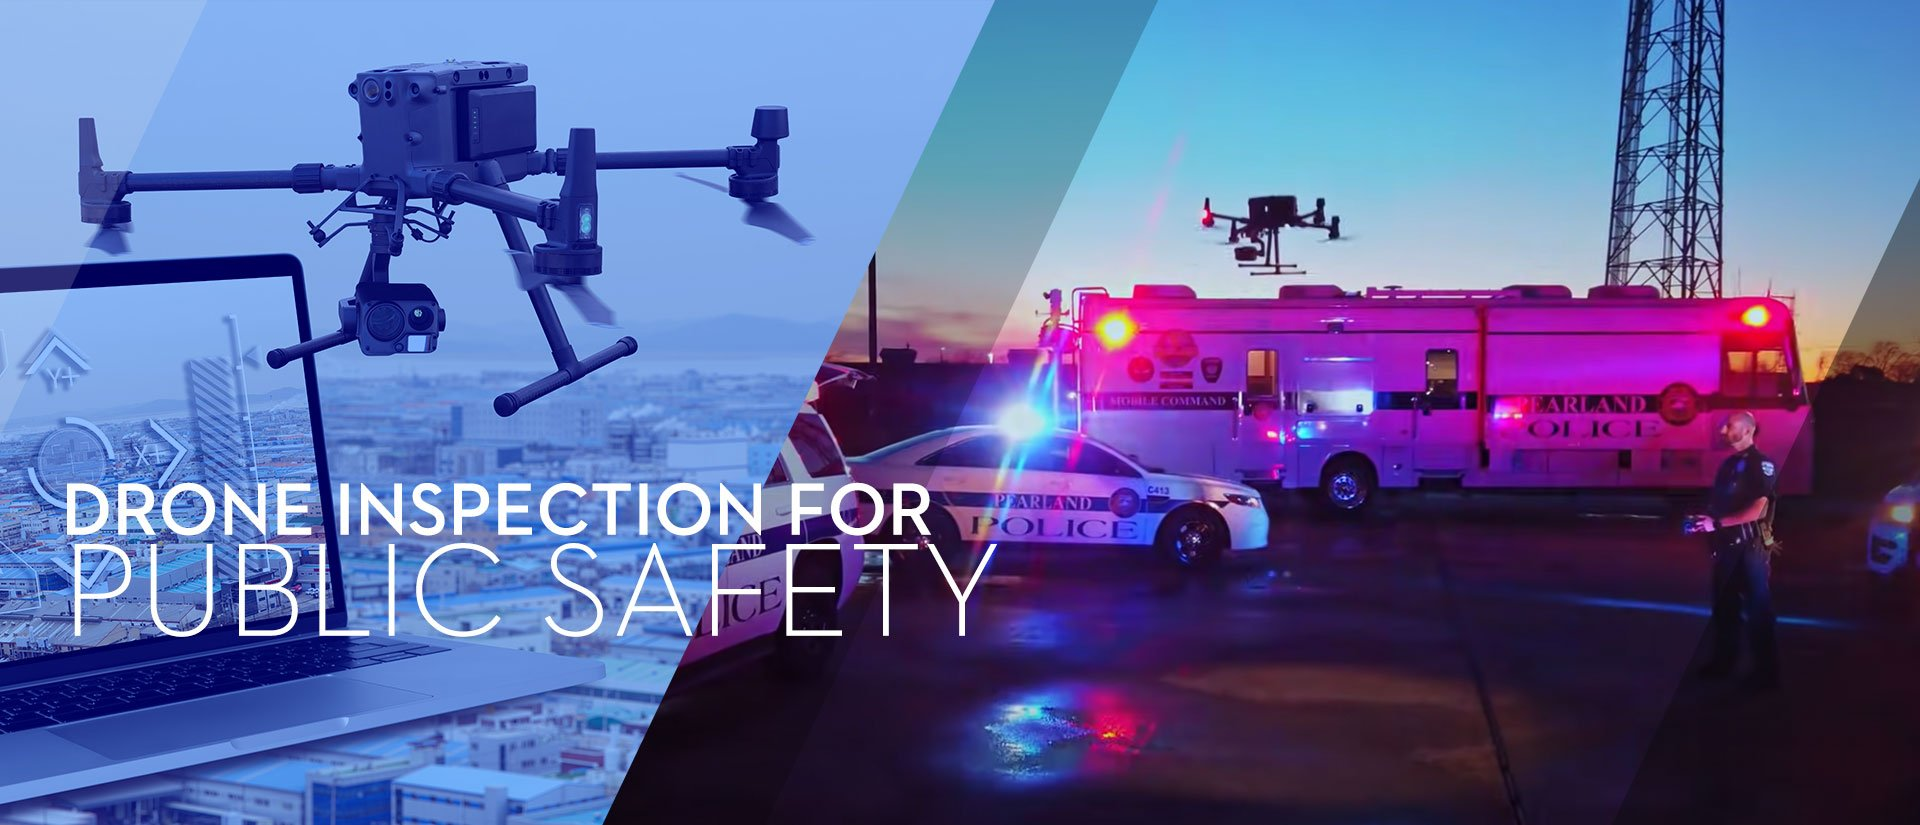
\includegraphics[width=0.45\textwidth,height=0.35\textheight]{DJI_B5}$^\dag$ 
  %\hfil
  %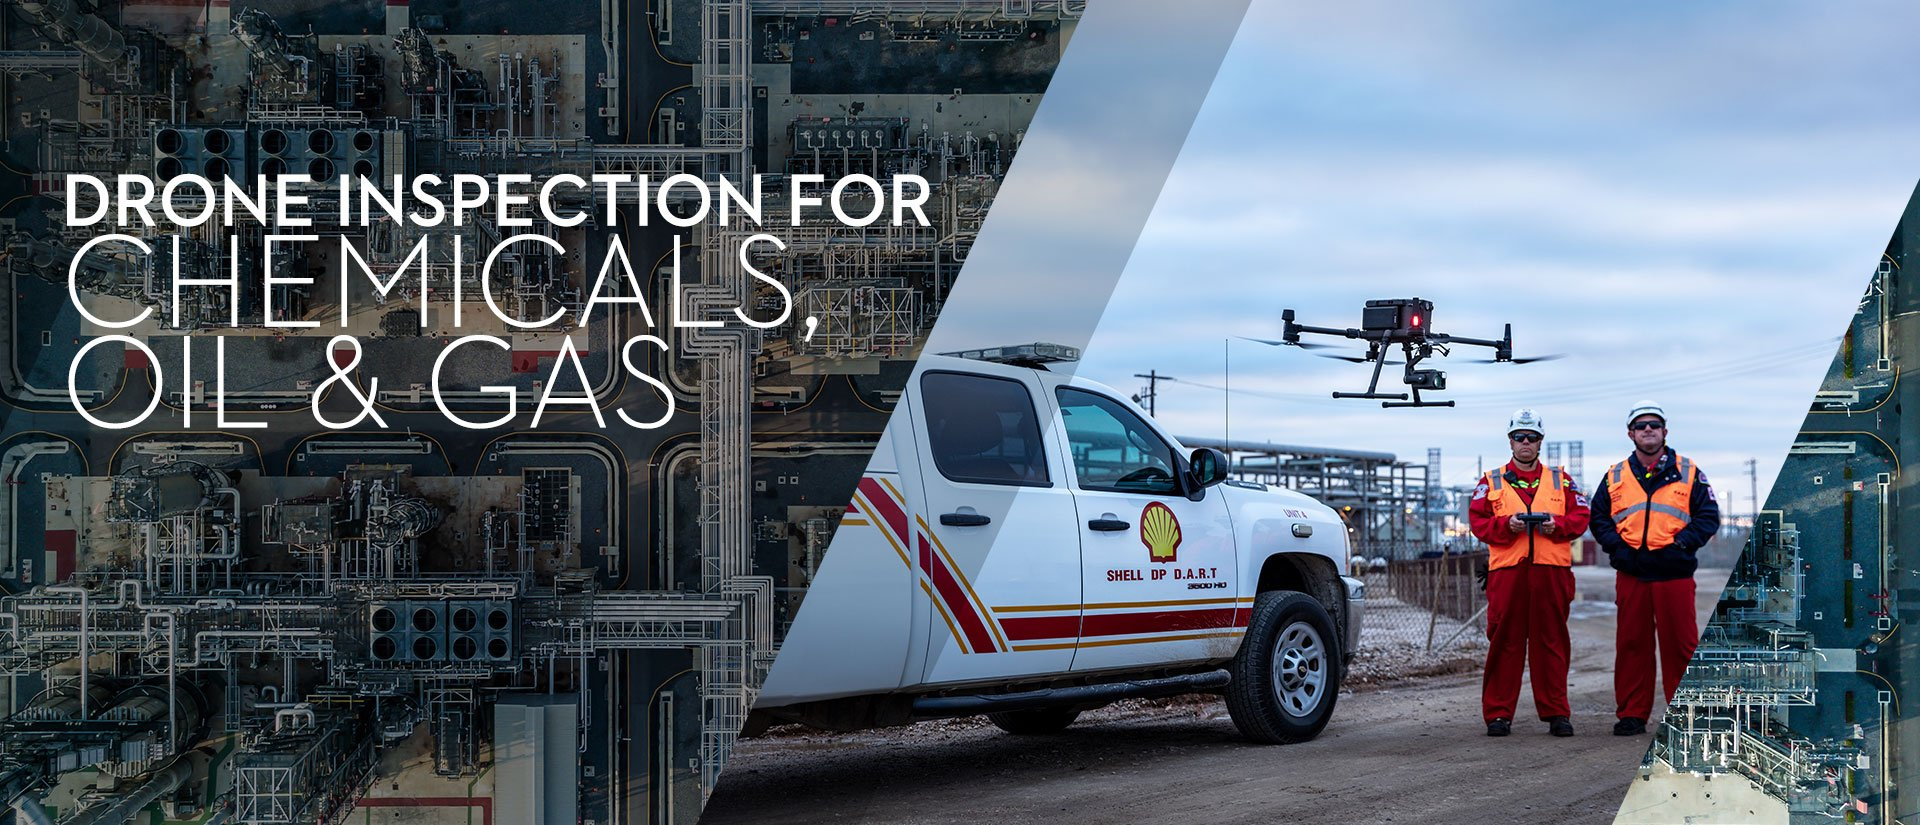
\includegraphics[width=0.45\textwidth,height=0.35\textheight]{DJI_B4}$^\dag$\\
  %\rule{0in}{1.2em}$^\dag$ \small Inspecciones con VANT basadas en los mejores casos de uso\\
  %\tiny \url{https://enterprise-insights.dji.com/blog/complete-guide-to-drone-inspections}
%\end{frame}

%\begin{frame}{Representacion 3D}
%  \bigskip % Vertical whitespace
  %\centering
%  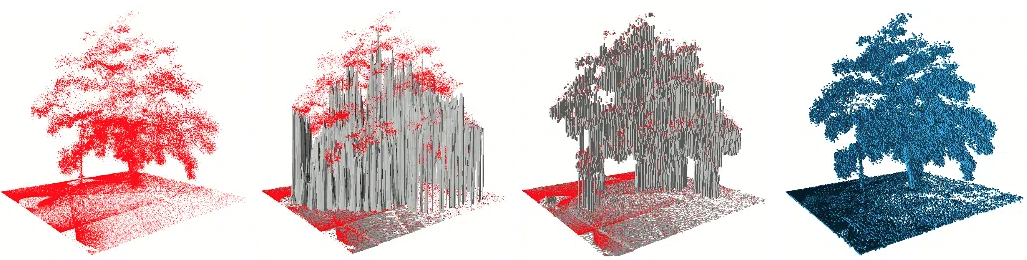
\includegraphics[width=1\textwidth,height=0.35\textheight]{img4}\footnotemark
%  \vspace{2pt}\\
%  \bigskip % Vertical whitespace
  
%  \begin{itemize}
%  \item Nube de puntos.
%  \item Mapa de elevación.
%  \item Superficies multi-nivel.
%  \item Octrees.
%  \end{itemize}
%  \footnotetext{OctoMap: An Efficient Probabilistic 3D Mapping Framework Based on Octrees [\cite{hornung13auro}]}
  
%\end{frame}

%\begin{frame}{Planificación de movimiento}
  
  %\centering
  %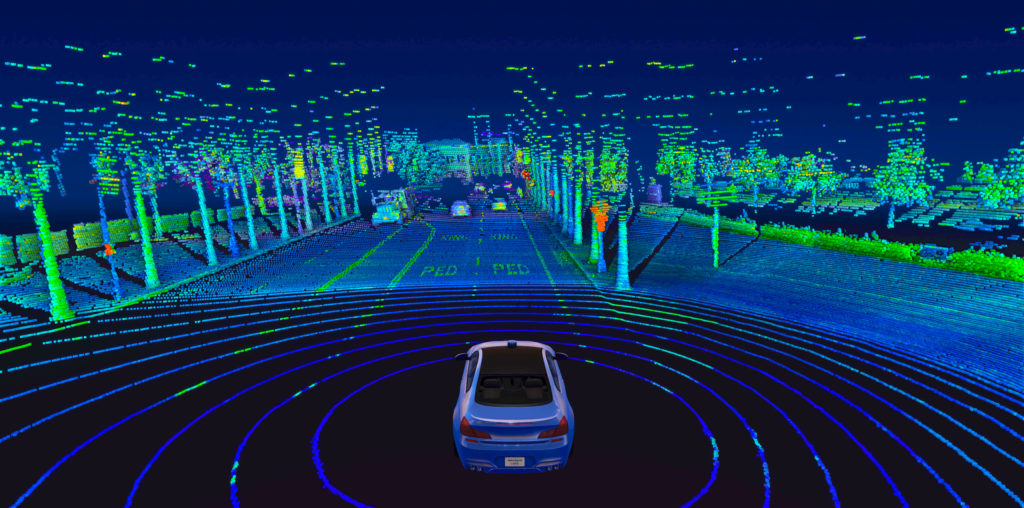
\includegraphics[width=0.45\textwidth,height=0.35\textheight]{map3d.jpg}$^\dag$
  %\hfil
  %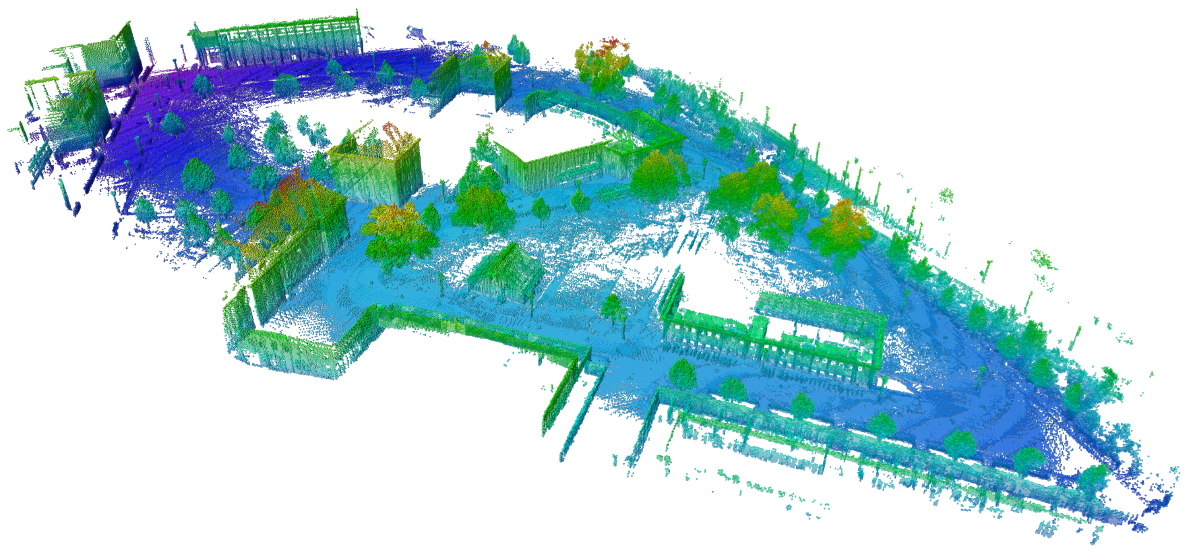
\includegraphics[width=0.45\textwidth,height=0.35\textheight]{map3d_2}$^\dag$
  %\vspace{2pt}\\
  %\bigskip % Vertical whitespace
%  Indica a un robot como moverse de un punto a otro en su entorno. Implica la generación de trayectorias y movimientos que permiten a los robots cumplir sus tareas o alcanzar sus objetivos mientras evitan obstáculos \footnotemark.\\
%  \bigskip % Vertical whitespace
%  \addvspace{\medskipamount}
%  \noindent
%  \begin{tabularx}{\linewidth}{ @{} X X @{} }
%    Por Grafos
    
%    \begin{itemize}
%    \item Grafos de visibilidad. 
%    \item Diagramas de Voronoi.
%    \item Descomposición por celdas.
%    \item Consulta única (RRT)
%    \item Consulta múltiple (PRM)
%    \end{itemize} &

%    Algoritmos
    
%    \begin{itemize}
%    \item BFS, DFS
%    \item A*, D*
%    \item Dijkstra
%    \end{itemize}
%  \end{tabularx}
%  \footnotetext{Different Cell Decomposition Path Planning Methods for Unmanned Air Vehicles A Review [\cite{Debnath2020}]}
%\end{frame}

\begin{frame}{Motivación del proyecto}
  \begin{minipage}{0.47\textwidth}

    \small La meta de este trabajo es la creación de una estrategia para la exploración de ambientes desconocidos de manera coordinada con múltiples vehículos aéreos no tripulados (VANTS).
    \bigskip % Vertical whitespace
    \begin{itemize}
    %\item Exploración con algoritmos de baja complejidad computacional.
    \item Búsqueda y rescate.
    \item Seguridad e Inspección
    \end{itemize}
  \end{minipage}
  \hspace{0.2cm}
  \begin{minipage}{0.5\textwidth}
    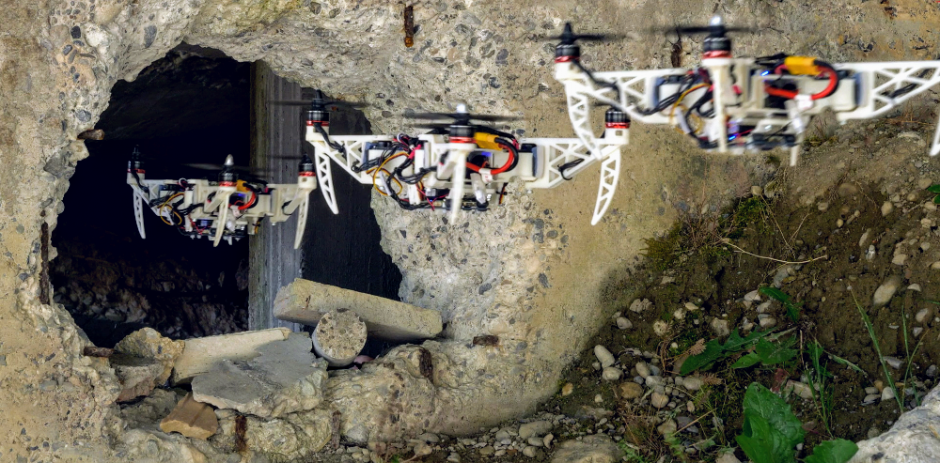
\includegraphics[width=\textwidth]{foldable-drone}$^\dag$\\
      \rule{0in}{1.2em}$^\dag$\scriptsize Foldable drone could aid search and rescue missions.\\
      \tiny \url{https://www.therobotreport.com/foldable-drone-could-aid-search-and-rescue-missions/} 
  \end{minipage}
\end{frame}

\section{Planteamiento del problema}
\begin{frame}
  \frametitle{Planteamiento del problema}
  \centering
  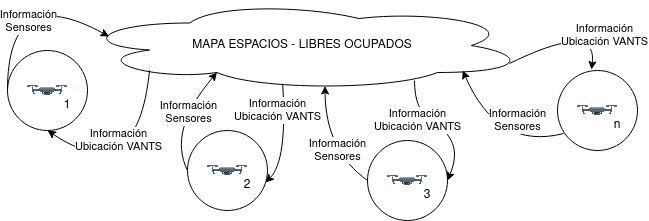
\includegraphics[width=10cm]{problema}
  %\begin{columns}
  %  \column{0.5\textwidth}
  %\justifying
  %\small Dado un volumen de interés desconocido en un espacio cerrado que se desea explorar denotada como $\mathcal{S}$, tal que $\mathcal{S} \subset \mathbb{R}^{3}$.\\
  %Encontrar y repartir rutas libres de colisiones para un conjunto de VANTS denotado como $\mathcal{V} = \{\mathcal{V}_{1},\mathcal{V}_{2},\mathcal{V}_{3},...,\mathcal{V}_{n}\}$ siendo $n$ el número total de VANTS disponibles, comenzando cada uno en un estado inicial conocido denotados como $q = \{q_{1},q_{2},q_{3},...,q_{n}\}$, y terminando en una configuración que maximice la localización del VANT y exactitud en la construcción del mapa.\\

  %La representación del volumen a explorar se utiliza un mapa de ocupación que se obtiene dividiendo el volumen en volumenes cúbicos (voxel) que puede tomar los valores de libre, ocupado y desconocido o no explorado de notados como $v_{libre}$, $v_{ocup}$, $v_{desc}$ con lecturas a partir de los valores de una cámara RGB-D basada en un modelo de ocupación probabilístico.\\

  
  
  \bigskip % Vertical whitespace
  El problema se basa en la propuesta de una estrategia que incluya las habilidades de autonomía para tareas de exploración de forma coordinada, dividiendo la carga de trabajo de exploración entre el grupo de VANTS.\\
  
  %Para lograr una exploraci\'{o}n eficiente y completa con un tiempo y recursos m\'{i}nimos, el problema requiere la creaci\'{o}n de algoritmos y t\'{e}cnicas de optimizaci\'{o}n.\\
    
  %\pause
  
  
   % \column{0.5\textwidth}\\
   % \pause
   % \centering
   % \small Retos multi-VANT
   % \begin{itemize}
   % \small \item Coordinación% - Establecer comunicación efectiva entre los múltiples VANTs. Intercambiar información relevante. Tener baja latencia en su comunicación.
   % \small \item Planificación% - Los VANTs deben coordinar sus movimientos para evitar colisiones y lograr una cobertura eficiente del área objetivo.
   % \small \item Asignación de tareas% - Se busca evitar la duplicación de esfuerzos optimizando el uso de recursos disponibles.
   % \end{itemize}
   %\end{columns}
\end{frame}

\section{Hipótesis y preguntas de investigación}

\begin{frame}{Hipótesis}

  Una estrategia que coordine y asigne tareas de exploración para múltiples VANTS, en combinación con una arquitectura de software (que resuelva los problemas de localización, manejo de mapas y planificación de rutas) mejorará el desempeño en tareas de exploración con múltiples VANTS en entornos desconocidos en interiores.
  
  %La implementación de una estrategia de exploración coordinada utilizando múltiples vehículos aéreos no tripulados (multi-VANT) en ambientes sin señal GPS, permitirá obtener mejores resultados en comparación con la exploración individual (mono-VANT). Esta coordinación eficiente se traducirá en una reducción del tiempo y los recursos necesarios para completar la exploración, así como en una mayor cobertura del área de interés. Además, se espera que la exploración coordinada multi-VANT mejore la calidad de los datos recopilados, lo que permitirá tomar decisiones más informadas y eficaces en diversos campos, como la cartografía, la vigilancia, el monitoreo y la respuesta a desastres naturales.
  
  %La implementación de una arquitectura descentralizada integrada de algoritmos para la detección y evasión de obstáculos, toma de decisiones, navegación e inteligencia colectiva para los múltiples VANTS. Así como un enfoque de fusión de datos que integre la información de los sensores de los múltiples VANTS, mejorará la efectividad y conducirá a mejores resultados de exploración en entornos dinámicos e inciertos, incluida una mayor cobertura del área explorada, una mejor recopilación de datos en comparación con un enfoque de un solo VANT.
  
\end{frame}

\begin{frame}{Preguntas de investigación}
  
  %\pause
  \begin{itemize}

  \item ¿Qué mecanismos de coordinación existen dentro de la literatura que podrían ayudar en resolver el problema de exploración multi-VANT?
  \item ¿Es posible que el uso de una estructura de datos como octree para representar la ocupación de un volumen, sea más eficiente que una representación usando una matriz cúbica?
    %\pause
  %\item ¿Qué efectiva será en seguir una estrategia de exploración basada en asignación de tareas en comparación con los resultados reportados en la literatura?
    %\pause
  \item ¿Qué características de la dinámica del robot se deben considerar en el simulador, para que los resultados se aproximen a los del mundo real?
    
  \end{itemize}
\end{frame}

\section{Objetivos}
\begin{frame}{Objetivos generales y particulares del proyecto}
  %\frametitle
  \begin{enumerate}
    %\item<1-> General \\
    \item General \\
    \bigskip
    Desarrollar una estrategia de exploración descentralizada que permita resolver los problemas de coordinación para múltiples VANTS en ambientes desconocidos.
    \pause
    \bigskip
    % \item<2-> Particulares\\
    \item Particulares\\
    
    \begin{itemize}
    \item Desarrollar una arquitectura de software que resuelva los problemas de autonomía para un VANT (localización, manejo de mapas y navegación).
    \item Crear un mecanismo de coordinación que asigne trayectorias libres de colisiones para la tarea de exploración.
    \item Realizar pruebas y simulaciones de la solución propuesta en entornos complejos, analizando la relación tiempo de exploración y cobertura del área de interés.
    \end{itemize}
  \end{enumerate}
\end{frame}

%Explicar con el cronograma
\section{Enfoque propuesto}
\begin{frame}{Enfoque propuesto}
%\small Siguiendo los objetivos anteriores, la metodolog\'{i}a propuesta se divide en tres etapas, que comenzaron en septiembre del 2023 y terminarán en agosto de 2024. A continuaci\'{o}n se detallan cada una de las actividades que se plantean realizar en cada etapa.

%\small \textbf{Etapa 1. An\'{a}lisis y dise\~{n}o de la soluci\'{o}n propuesta}\\
%\small Esta etapa comprende la revisi\'{o}n de la literatura de manera m\'{a}s completa, que permita contar con la informaci\'{o}n necesaria para la elecci\'{o}n de los mejores algoritmos para abordar cada una de las problem\'{a}ticas asociadas con la coordinaci\'{o}n de múltiples robots en tareas de exploración, detectando áreas de oportunidad para el desarrollo de una estrategia descentralizada de coordinación. \\
%\bigskip
%\small \textbf{Etapa 2. Implementaci\'{o}n y validaci\'{o}n}\\
%\small Esta etapa se centra en el desarrollo e implementaci\'{o}n del dise\~{n}o de la arquitectura de software para la coordinaci\'{o}n multi-VANT, utilizando una herramienta de simulación de robots de libre acceso, cumpliendo estándares de modularidad de diseño.\\
%\bigskip
%\small \textbf{Etapa 3. Evaluaci\'{o}n experimental, resultados y conclusiones}\\
%\small Partiendo del prototipo y las simulaciones desarrolladas en la etapa anterior, en esta etapa se realizan todas las actividades relacionadas con la evaluación, compilación y análisis de los resultados.

    
  \begin{minipage}{0.47\textwidth}
    
    \begin{itemize}
      %\item Exploración con algoritmos de baja complejidad computacional.
    \item \small Probabilistic Road-Map (Método a base de muestreos) \footnote{Survey of UAV motion planning [\cite{Quan2020}]}  
    \item \small RGB-D $\implies$ Voxels $\implies$ Octomap
      
    \item \small Exploración basada en fronteras \footnote{A frontier-based approach for autonomous exploration [\cite{613851}]}
    \item \small Estrategia basada en auto-ofertas (Método Húngaro) \footnote{Estrategia descentralizada para la exploración multi-robot, incluyendo restricciones en rango de comunicación [\cite{LEAL2013}]}
      
    \end{itemize}
  \end{minipage}
  \hspace{0.1cm}
  \begin{minipage}{0.5\textwidth}
    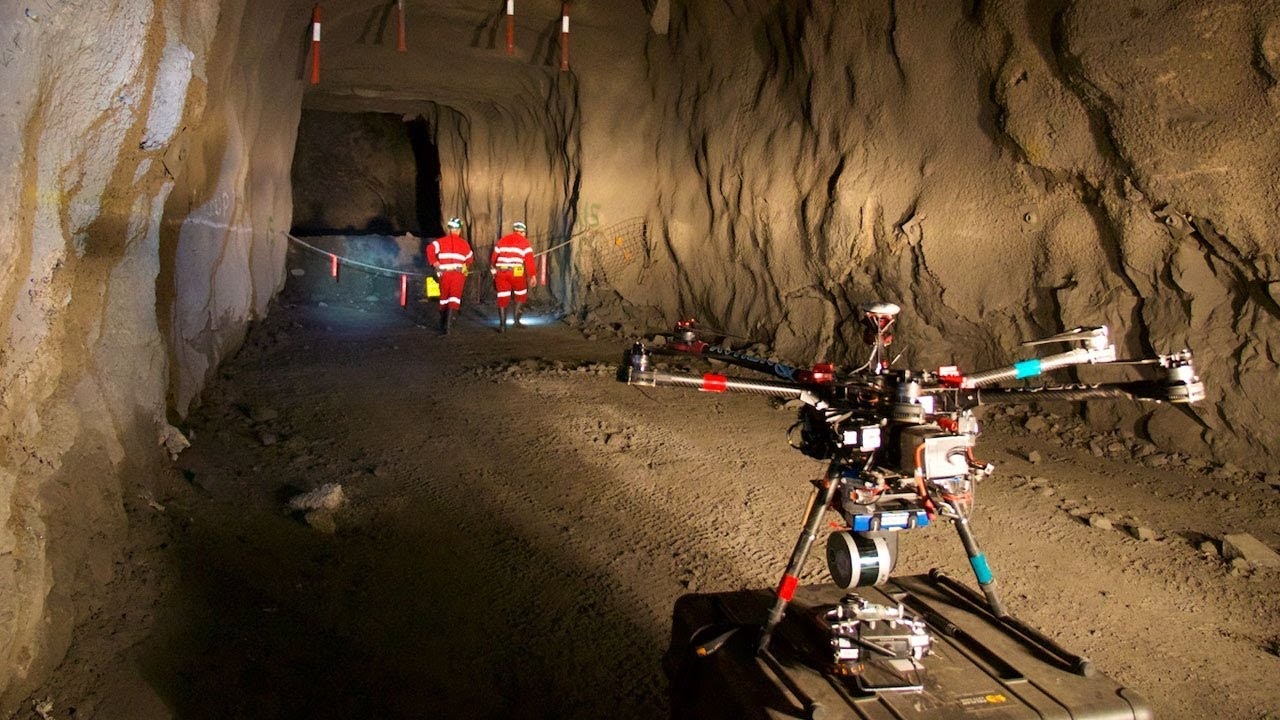
\includegraphics[width=\textwidth]{maxresdefault.jpg}$^\dag$\\
    \rule{0in}{1.2em}$^\dag$\scriptsize Ilustración Drone en Mina \\
    \tiny \url{https://dronevideos.com/} 
  \end{minipage}
  
\end{frame}

\begin{frame}{Estrategia \footnote{Estrategia descentralizada para la exploración multi-robot, incluyendo restricciones en rango de comunicación [\cite{LEAL2013}]}}

  
  
  \begin{minipage}{0.67\textwidth}
    \begin{itemize}
    \item[] \textcolor{teal}{Buscar que cada VANT se dirija hacia las fronteras más cercanas tratando de minimizar las distancias recorridas.}
      \bigskip % Vertical whitespace
    \item[] \textcolor{red}{Buscar la separación de los VANTS con la finalidad de minimizar el trabajo redundante y la interferencia entre ellos.}
      \bigskip % Vertical whitespace
    \item[] \textcolor{blue}{Mantener los VANTS en comunicación con los demás miembros del equipo actualizados y en caso de falla de algún VANT evitar que se pierda la información.}
    \end{itemize}
  \end{minipage}
  \hspace{0.6cm}
  \begin{minipage}{0.2\textwidth}
    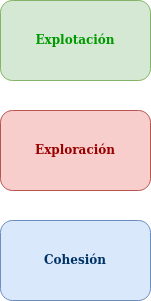
\includegraphics[width=1\textwidth]{estrategia}
  \end{minipage}
  
\end{frame}

\begin{frame}{Arquitectura}
  \begin{figure}
    \centering
    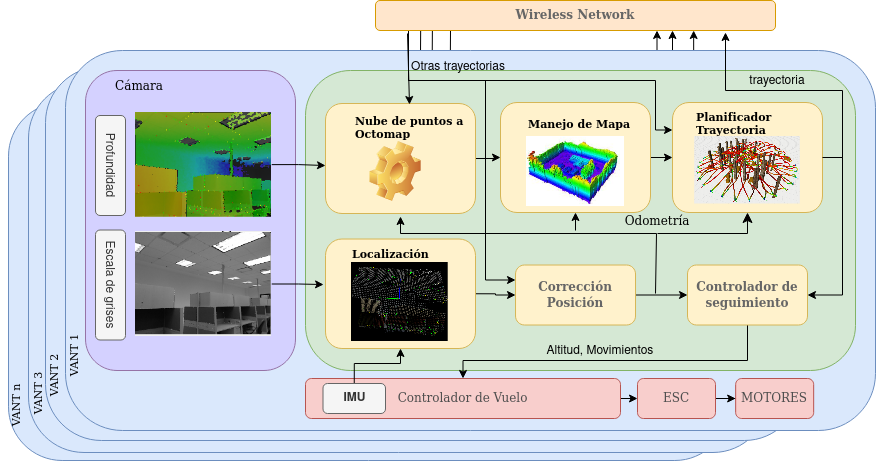
\includegraphics[width=15cm]{arquitectura}
  \end{figure}
\end{frame}

\begin{frame}{Robot Operating System (ROS)}


  \textbf{¿Qué es ROS?}\\
  \bigskip % Vertical whitespace
  \begin{itemize}
  \item Provee un conjunto de herramientas usadas por un robot (Sensores, actuadores, implementación diversos algoritmos)
  \item Framework de comunicación que permite interconectar las diferentes piezas del cerebro para hablar con otras lecturas de sensores.
  \end{itemize}
  \bigskip % Vertical whitespace
  En resumen ROS ayuda en descomponer software complejos en pequeñas piezas más manejables.
  
\end{frame}

\begin{frame}
  \begin{figure}
    \centering
    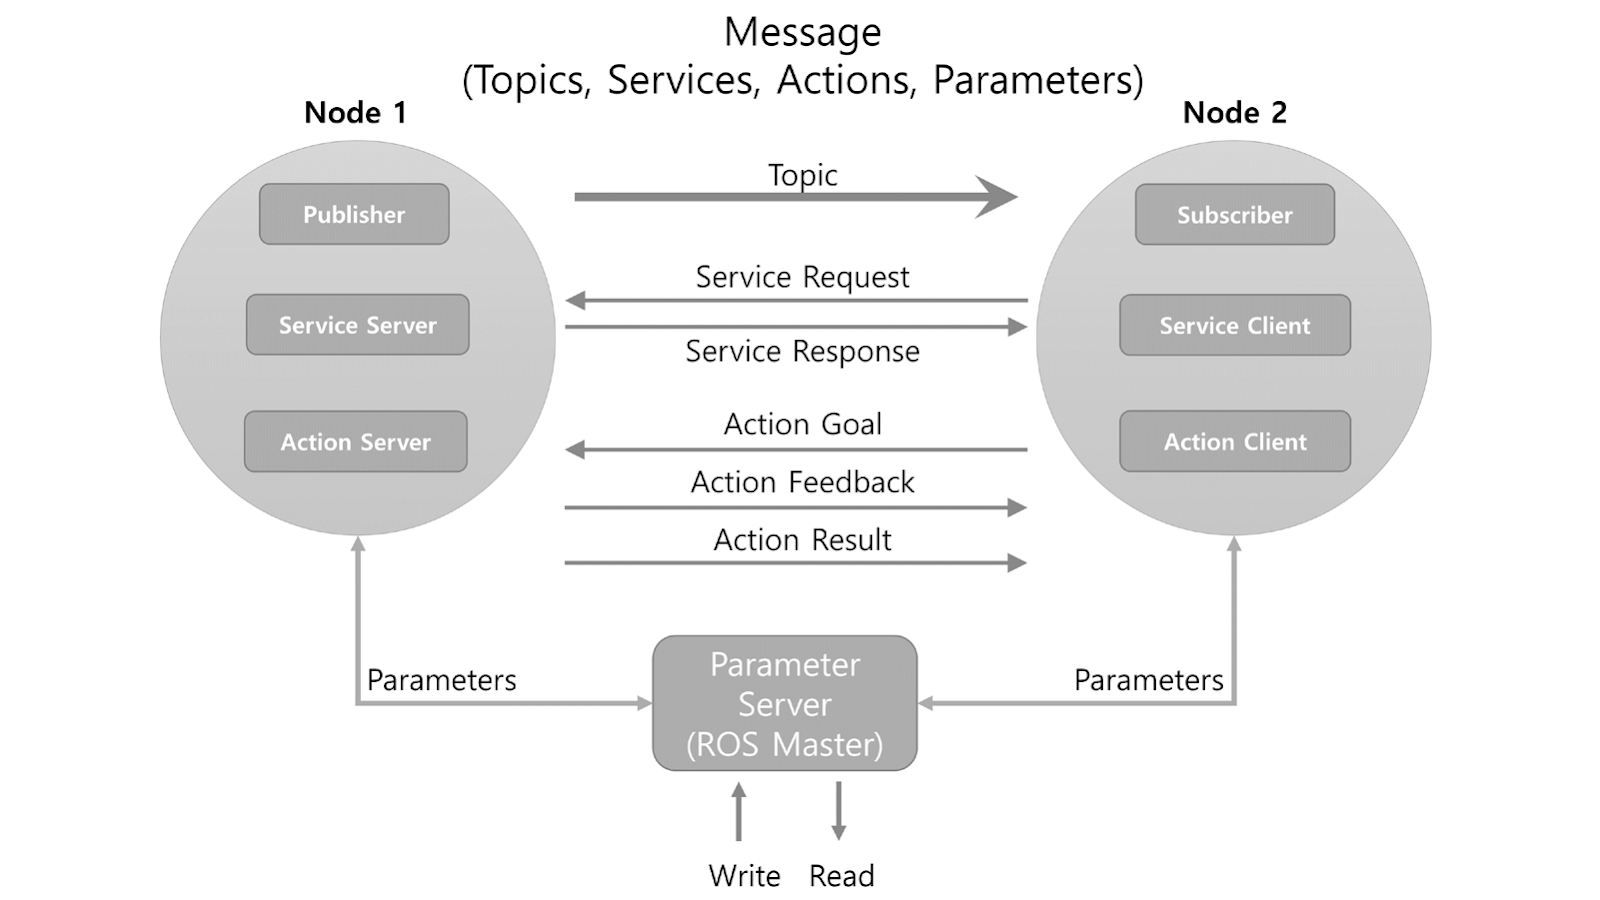
\includegraphics[width=0.75\textwidth]{ros_1}
  \end{figure}
\end{frame}

\begin{frame}{Simulador -  ROS Visualization (RVIZ) }
  \begin{figure}
    \centering
    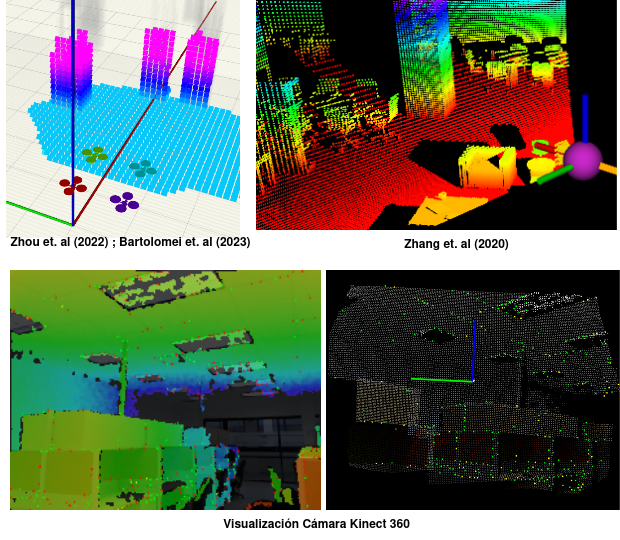
\includegraphics[width=0.57\textwidth]{visual}
  \end{figure}
\end{frame}

\begin{frame}{Marco experimental}

  El problema a considerar en el trabajo, es el reducir el tiempo de exploración en un ambiente desconocido con ayuda de múltiples VANTS.
  \bigskip % Vertical whitespace

  Edificios
  \begin{itemize}
    \item Oficina1
    \item Oficina2
    \item Oficina3
    \item Pilares
  \end{itemize}
  
  Bosques (50$m^{2}$)
  \begin{itemize}
    \item Bosque disperso (0.1 árboles/$m^{2}$)
    \item Bosque densidad media (0.15 árboles/$m^{2}$)
    \item Bosque denso (0.2 árboles/$m^{2}$)
    \item Bosque con múltiples densidades (4 densidades diferentes) 
  \end{itemize}
  
\end{frame}

\begin{frame}{Superficies a explorar}
  \begin{figure}
    \centering
    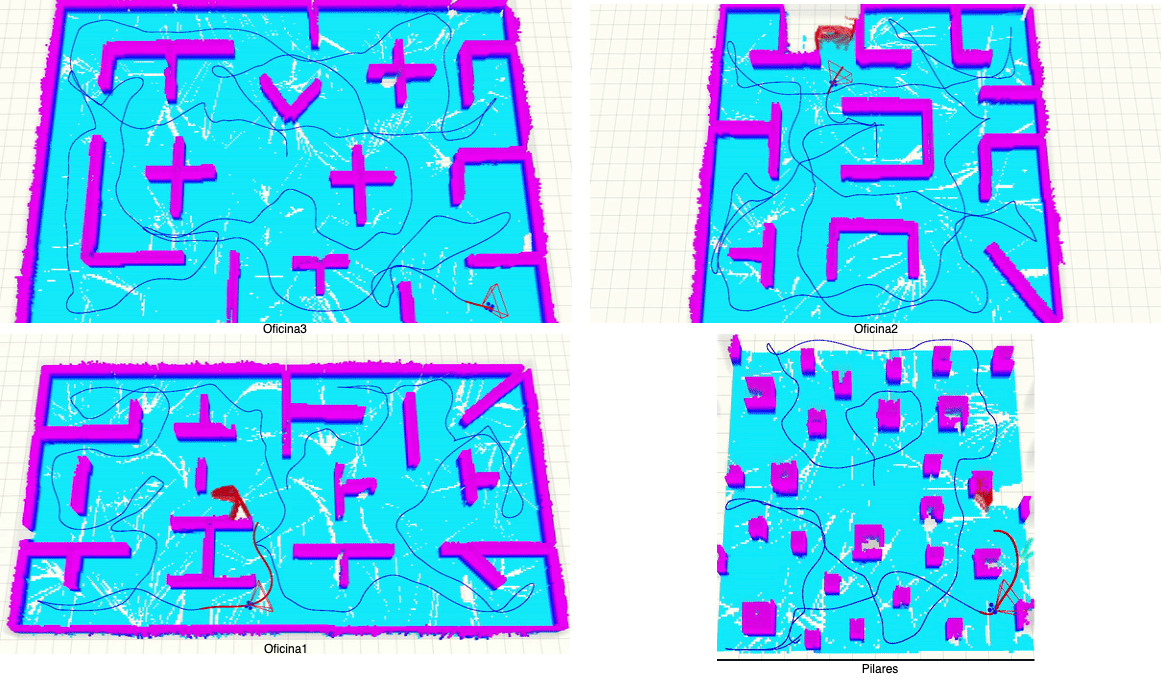
\includegraphics[width=0.75\textwidth]{pruebas}
  \end{figure}
\end{frame}

\begin{frame}{Validación de enfoque}

  El simulador dinámico \cite{RACER2022} \footnote{Rapid Collaborative Exploration With a Decentralized Multi-UAV System} utiliza la odometría de referencia de los VANTS, suponiendo que cada agente está equipado con una cámara de profundidad que mira hacia adelante cuya resolución es 640x480px y un campo de visión de 80°x60°. Las imágenes de profundidad se generan utilizando el proceso presentado en \cite{OMNI2022} \footnote{Omni-Swarm: A Decentralized Omnidirectional Visual–Inertial–UWB State Estimation System for Aerial Swarms} con un rango máximo de detección de 4.5 m.
  \bigskip % Vertical whitespace
  \begin{itemize}
  \item En tiempo necesario para completar la exploración del ambiente dado y la velocidad promedio de los VANTS durante cada experimento.
  \item Tasas de exploración para diferentes cantidades de VANTS en diversos ambientes.
  \end{itemize}
  
  
\end{frame}

\begin{frame}{Técnicas a comparar resultados}

  \begin{itemize}
  \item RACER: Rapid Collaborative Exploration With a Decentralized Multi-UAV System, \footnote{\cite{RACER2022}}
  \item FAST: Fast Multi-UAV Decentralized Exploration of Forests \footnote{\cite{BARTOLOMEI2023}}
  \end{itemize}
  
\end{frame}

\begin{frame}[allowframebreaks,noframenumbering]{Bibliografía}
  \tiny
  \bibliographystyle{abbrvnat}
  \bibliography{test}
\end{frame}

\end{document} 
